
% Folie: Fachschaftsmodul Git / Versionierung
\begin{frame}
    \centering
    \begin{figure}[H]
        \includegraphics[keepaspectratio, width=.5\paperwidth, height=\paperheight]{Logos/FreeFlower.pdf}
    \end{figure}
    \large \textbf{Arbeiten planen, organisieren und versionieren mit \texttt{git}}
\end{frame}

% Lernziele
\begin{frame}[fragile]{Lernziele}
    \begin{itemize}
        \item[\faSquare] Sie können eine grössere Arbeit in Teilaufgaben zerlegen
        \item[\faSquare] Sie verstehen, warum Versionierung wichtig ist
        \item[\faSquare] Sie kennen einfache Git-Grundkonzepte und bewährte Arbeitsweisen
        \item[\faSquare] Sie können Ihre Maturaarbeit technisch sauber organisieren
    \end{itemize}
\end{frame}

% 1. Einstieg: Das Problem
\begin{frame}{1. Einstieg: Das Problem (10 min)}
    \centering
    \begin{block}{Beispielgeschichte}
        \texttt{Maturaarbeit.docx}\\\pause
        \texttt{Maturaarbeit\_final.docx}\\\pause
        \texttt{Maturaarbeit\_final2.docx}\\\pause
        \texttt{Maturaarbeit\_final\_wirklich\_final.docx}
    \end{block}
    \pause
    \vspace{0.6em}
    \begin{itemize}
        \item Wenn Sie etwas nicht reproduzieren können, haben Sie es nicht sauber dokumentiert.
        \item Was passiert bei einem Fehler?
        \item Wie arbeiten Sie zusammen?
    \end{itemize}
\end{frame}

% 2. Projektorganisation allgemein
\begin{frame}{2. Projektorganisation allgemein}{Zerlegung des Problems in grobe Schritte mit GANTT-Chart}
    \textbf{GANTT-Charts}: Projektzeitplan, Aufgaben und Abhängigkeiten. Zeitleiste mit Balken für Aufgaben, Meilensteine, Ressourcenplanung. Hilft bei Planung, Überwachung und Kommunikation von Fortschritt.
    \begin{figure}
        \centering
        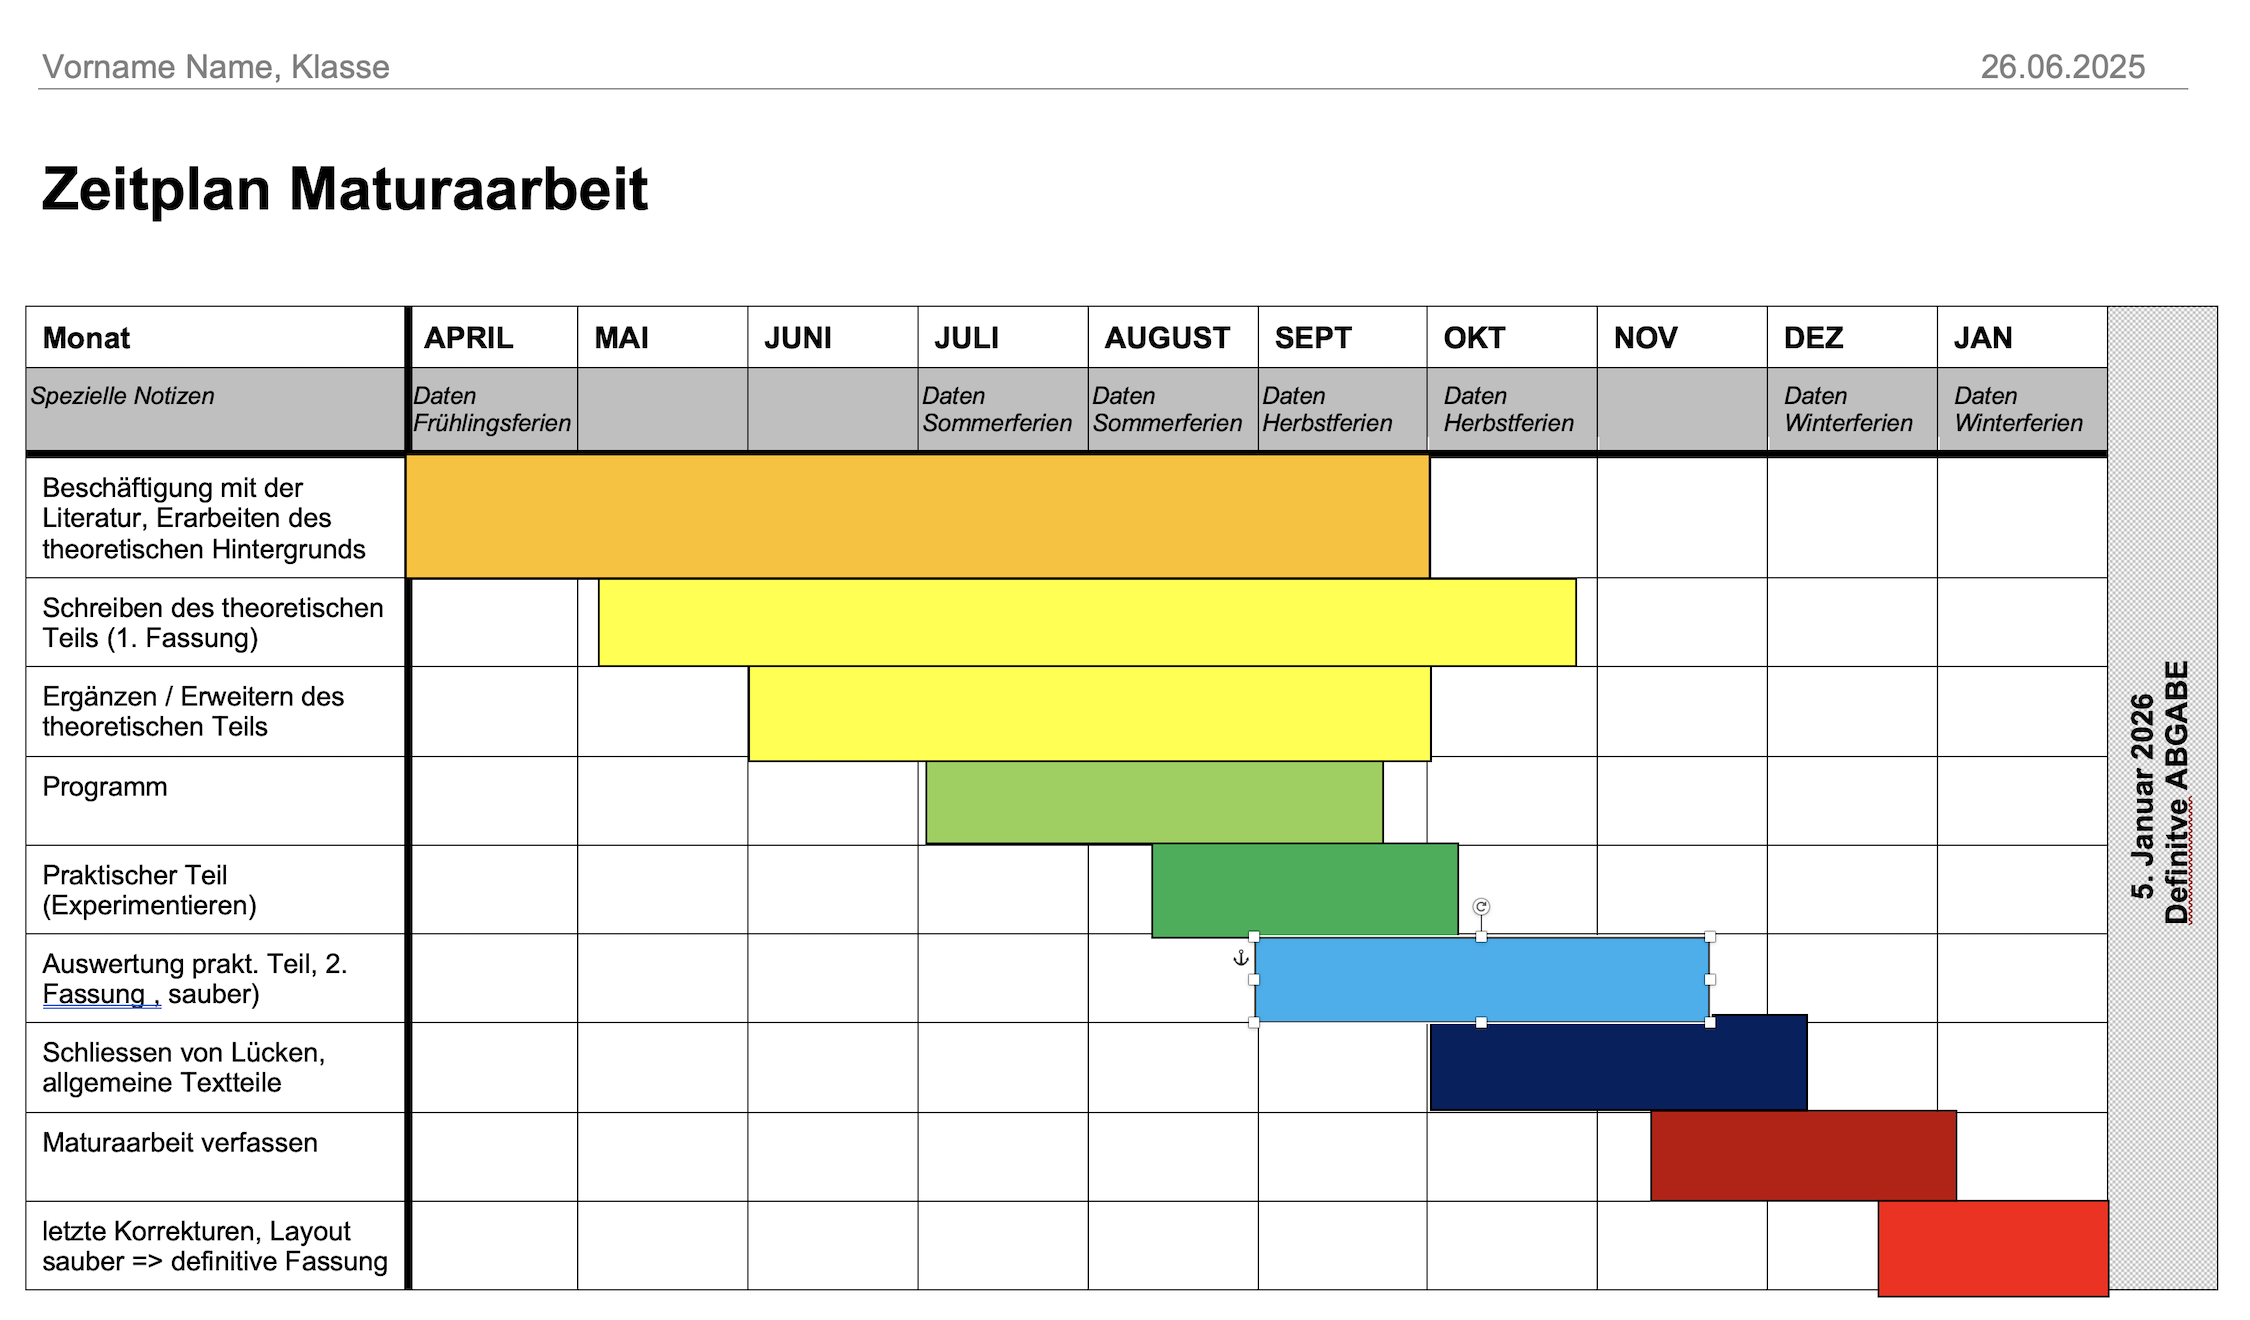
\includegraphics[width=\textwidth]{Various/Fachschaftsmodule/Gantt-Chart.png}
    \end{figure}
\end{frame}

\begin{frame}
    \begin{myExBox}[title=Übung: GANTT-Chart für die Maturaarbeit erstellen]
        Erstellen Sie einen einfachen GANTT-Chart mit den Hauptschritten Ihrer Maturaarbeit (Recherche, Datenaufbereitung, Schreiben, Revision) und planen Sie die zeitliche Abfolge über die nächsten Monate. Berücksichtigen Sie dabei auch Pufferzeiten für unerwartete Verzögerungen.
        \tcblower
        \textbf{Ziel}: Klarer Überblick über die zeitliche Planung und Abfolge der Arbeitsschritte.
    \end{myExBox}
\end{frame}

\begin{frame}
    \begin{center}
        Aber wann mache ich genau was? \sout{To-Do-Liste} \pause Kalender!
    \end{center}
\end{frame}

% Kalender-Layer für Planung
\begin{frame}[fragile]{Kalender-Layer für Planung}
    \begin{block}{Kurz}
        Statt To-Do-Listen in Dateien oder Issues: Kalender-Layer mit wöchentlichen Tasks für die einzelnen Arbeitsschritte (Recherche, Datenaufbereitung, Schreiben, Revision). Sichtbare Wochenplanung, klare Zeitfenster pro Arbeitsschritt, einfache Nachverfolgbarkeit.
    \end{block}
\end{frame}
\begin{frame}
    \centering
    \begin{figure}[H]
        \centering
        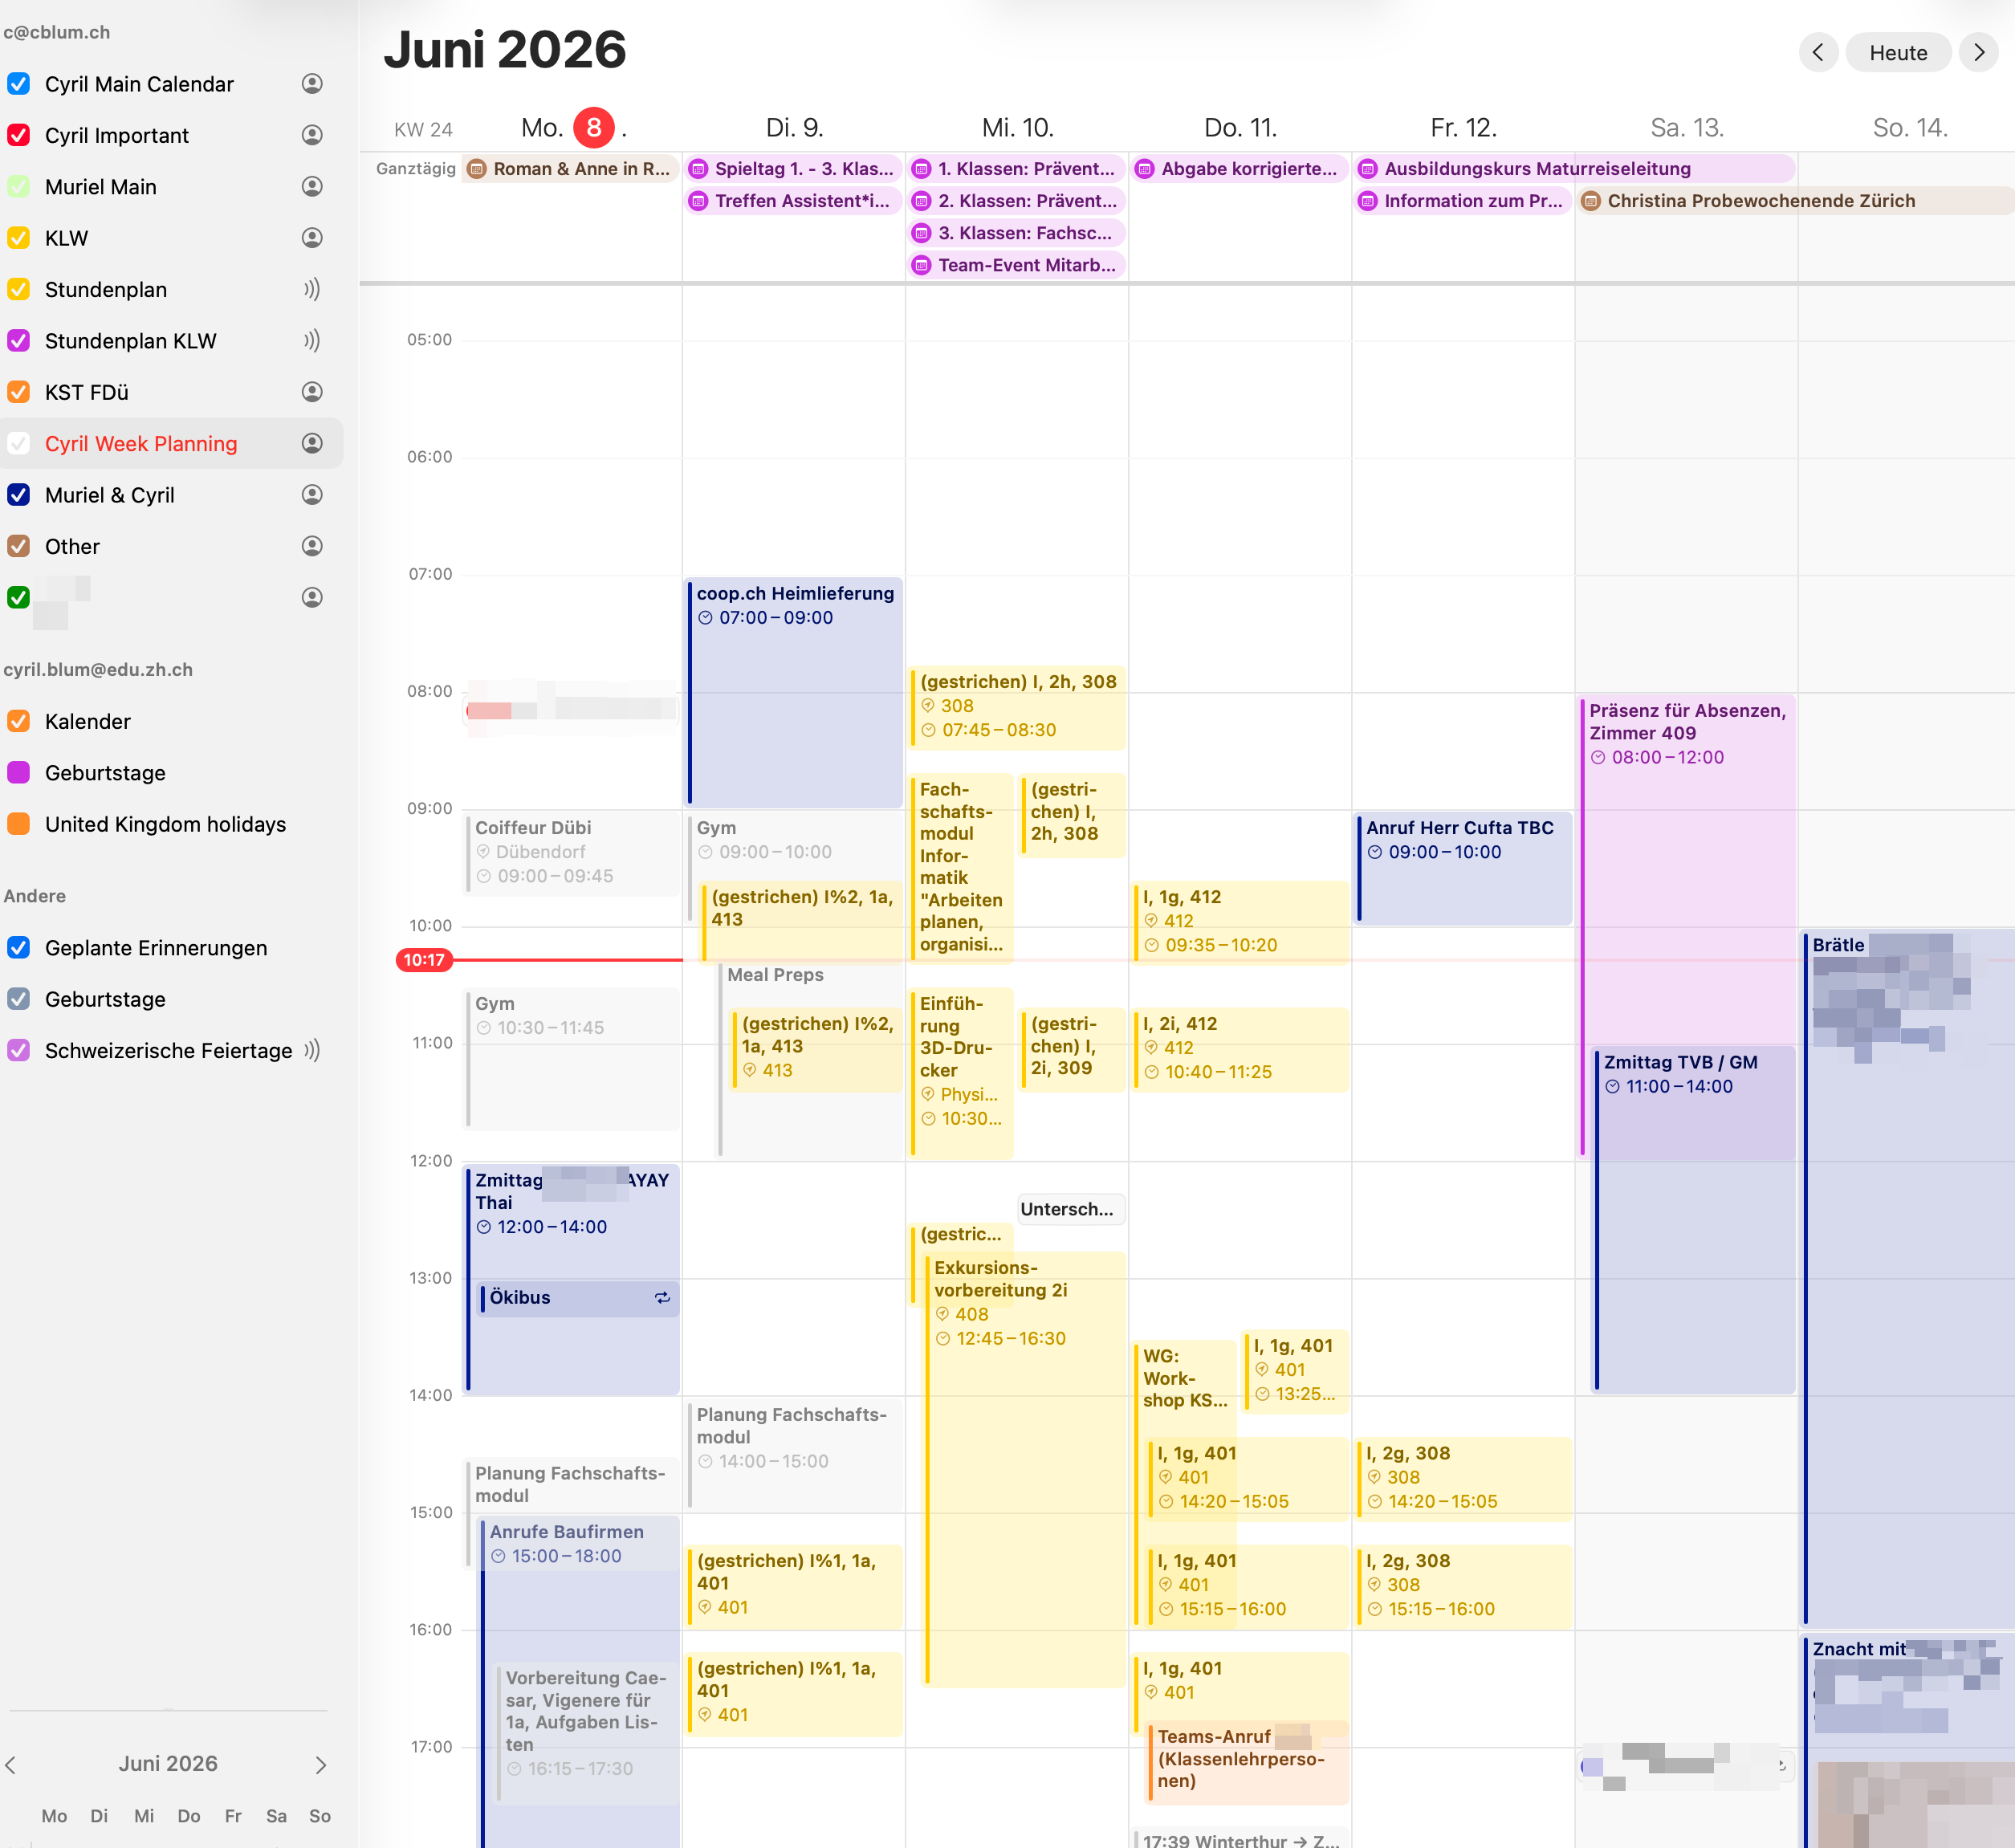
\includegraphics[width=\textwidth]{Various/Fachschaftsmodule/Calendar-Planning.png}
    \end{figure}
    \vspace{0.6em}

\end{frame}

\begin{frame}{Übung: Eigenen Kalender-Layer anlegen}
    \begin{myExBox}[title=\emoji{calendar} Übung: Kalender-Layer anlegen]
        Legen Sie einen neuen Kalender-Layer mit dem Namen \textbf{Week Planning} an und erstellen Sie für die nächsten 8 Wochen wöchentliche, wiederkehrende Termine für die einzelnen MA-Schritte (Recherche, Datenaufbereitung, Schreiben, Revision).\\[0.6em]
        \small \textit{\emoji{pen} Alternativ (auf Papier)}: Zeichnen Sie eine einfache Wochenübersicht und planen Sie die nächsten 8 Wochen mit den Hauptschritten Ihrer Maturaarbeit.
        \tcblower
        \textbf{Ziel}: Sichtbare Wochenplanung, klare Zeitfenster pro Arbeitsschritt, einfache Nachverfolgbarkeit.
    \end{myExBox}
\end{frame}


\begin{frame}{2. Projektorganisation allgemein}{Ordnerstruktur und Dokumentation}
    \centering
    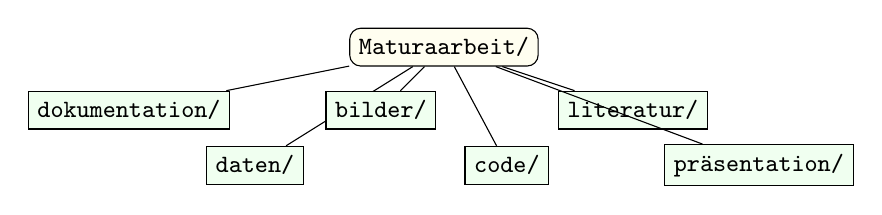
\begin{tikzpicture}[level distance=8mm, sibling distance=16mm, every node/.style={font=\small\ttfamily}]
        \node[draw, rectangle, rounded corners, fill=yellow!6] (root) {Maturaarbeit/}
        child { node[draw, rectangle, fill=green!6] {dokumentation/} }
        child { node[draw, rectangle, fill=green!6, yshift=-7mm] {daten/} }
        child { node[draw, rectangle, fill=green!6] {bilder/} }
        child { node[draw, rectangle, fill=green!6, yshift=-7mm] {code/} }
        child { node[draw, rectangle, fill=green!6] {literatur/} }
        child { node[draw, rectangle, fill=green!6, yshift=-7mm] {präsentation/} };
    \end{tikzpicture}
    \vspace{0.6em}
    \begin{block}{Kernpunkte}
        Konsistente Ordnerstruktur, sinnvolle Dateinamen, Backups separat von Versionierung, Rohdaten nie überschreiben.
    \end{block}
    \vspace{0.4em}
    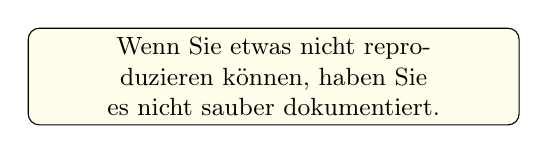
\begin{tikzpicture}[every node/.style={draw, rounded corners, fill=yellow!8, align=center, font=\small, text width=6cm}, node distance=6mm]
        \node (p) {\enquote{Wenn Sie etwas nicht reproduzieren können, haben Sie es nicht sauber dokumentiert.}};
    \end{tikzpicture}
\end{frame}
\begin{frame}[fragile]{Aufgabe}
    \begin{myExBox}[title=Aufgabe: Ordnerstruktur und Dokumentation anlegen]
        \scriptsize
        Legen Sie eine konsistente Ordnerstruktur für Ihre Maturaarbeit an (z.\,B. \texttt{dokumentation/}, \texttt{daten/}, \texttt{code/}, \texttt{literatur/}, \texttt{präsentation/}). 
        
        Erstellen Sie eine kurze Dokumentation (z.\,B. in einer \texttt{README.md}), z.B.::

        \begin{lstlisting}[style=bash, basicstyle=\color{white}\ttfamily\scriptsize, breaklines=true]
# Maturaarbeit: Titel der Arbeit
## Ordnerstruktur
- dokumentation/: Alle Dokumente, Berichte, Protokolle
- daten/: Rohdaten, Aufbereitete Daten
- code/: Alle Skripte, Jupyter Notebooks
- literatur/: Alle Literaturquellen, PDFs, Zitate
- präsentation/: Alle Präsentationsdateien, Folien, Grafiken
## Dokumentation
- Alle Schritte der Datenaufbereitung, Analyse und Ergebnisse werden hier dokumentiert.
        \end{lstlisting}
        MarkDown-Syntax: \url{https://www.markdownguide.org/basic-syntax/}
        
        Legen Sie einen separaten Ordner für Backups an und stellen Sie sicher, dass Rohdaten nicht überschrieben werden.
    \end{myExBox}
\end{frame}


% Warum Versionierung?
\begin{frame}{Warum Versionierung?}
    \begin{center}
        \begin{tikzpicture}[node distance=18mm, every node/.style={font=\small}]
            \node[draw, rounded corners, fill=blue!10] (safety) {Sicherheit};
            \node[draw, rounded corners, fill=green!10, right=of safety] (history) {Historie};
            \node[draw, rounded corners, fill=orange!10, right=of history] (collab) {Zusammenarbeit};
            \node[draw, rounded corners, fill=purple!10, below=of history] (experiment) {Experimentieren\ \footnotesize(Branching)};
            \draw[->, thick] (safety) -- (history);
            \draw[->, thick] (history) -- (collab);
            \draw[->, thick, dashed] (collab) -- (experiment);
        \end{tikzpicture}
    \end{center}
\end{frame}

% Einfache Arbeitsroutine
\begin{frame}[fragile]{Einfacher Workflow}
    \centering
    \begin{tikzpicture}[node distance=16mm, every node/.style={font=\small}]
        \node[draw, rounded corners, fill=gray!10] (work) {Arbeiten lokal};
        \node[draw, rounded corners, fill=green!10, right=of work] (commit) {Commit};
        \node[draw, rounded corners, fill=blue!10, right=of commit] (push) {Push zum Remote};
        \draw[->, thick] (work) -- (commit);
        \draw[->, thick] (commit) -- (push);
    \end{tikzpicture}
\end{frame}

% Commit-Graph
\begin{frame}{Commit-Graph (visuell)}
    \centering
    \begin{tikzpicture}[x=11mm, y=10mm, commit/.style={circle, draw, inner sep=1.2pt, font=\scriptsize\ttfamily, minimum size=6mm}, node distance=12mm, on grid]

        \node[commit] (m1) at (0,1) {m\textsubscript{1}};
        \node[commit, right=of m1] (m2) {m\textsubscript{2}};
        \node[commit, right=of m2] (m3) {m\textsubscript{3}};
        \node[commit, right=of m3] (m4) {m\textsubscript{4}};
        \node[commit, right=of m4] (m5) {m\textsubscript{5}};
        \begin{scope}[on background layer]
            \node[fit=(m1) (m5), draw=black, fill=blue!10, rounded corners, label={[xshift=4pt]right:\small\texttt{main}}, dotted, inner xsep=10pt, inner ysep=5pt] {};
        \end{scope}

        \node[commit, below right=2cm and .5cm of m2] (f1) {f\textsubscript{1}};
        \draw[->, dashed, thick] (m2) -- node[midway, left, font=\scriptsize, draw=none] {add branch} (f1);
        \node[commit, right=of f1] (f2) {f\textsubscript{2}};
        \node[commit, right=of f2] (f3) {f\textsubscript{3}};

        \draw[->, thick] (m1) -- (m2) -- (m3) -- (m4) -- (m5);
        \draw[->, thick] (f1) -- (f2) -- (f3);


        \begin{scope}[on background layer]
            \node[fit=(f1) (f3), draw=black, fill=green!10, rounded corners, label={[xshift=4pt]right:\small\texttt{feature/x}}, dotted, inner xsep=10pt, inner ysep=5pt] {};
        \end{scope}
        % for curved arrow: .. controls +(0,.75) and +(0,-.75) .. 
        \draw[->, thick] (f3) -- node[midway, right, font=\scriptsize, draw=none] {PR / Merge} (m5);
    \end{tikzpicture}
    \pause
    \begin{center}
        Beispiel: \url{https://github.com/CyrilBlum/FreeFlower}
    \end{center}
\end{frame}

\begin{frame}[fragile]{Unterschiede visualisieren}
    \begin{figure}[H]
        \centering
        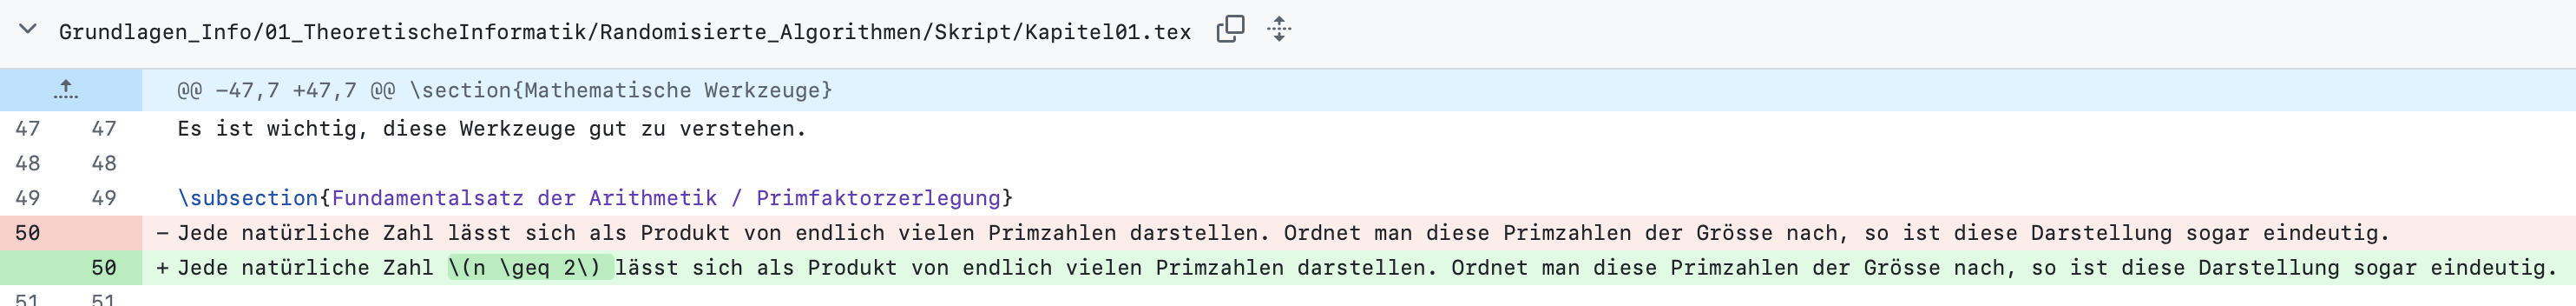
\includegraphics[width=\textwidth]{Various/Fachschaftsmodule/Diff-Visualisierung.png}
    \end{figure}
    \begin{center}
        Demo auf GitHub: \url{https://github.com/CyrilBlum/FreeFlower}
    \end{center}
\end{frame}

% Remote Zusammenarbeit
\begin{frame}{Zusammenarbeit: Remote (Push / Pull)}
    \centering
    \begin{tikzpicture}[node distance=22mm, every node/.style={font=\small}]
        \node[draw, cylinder, cylinder uses custom fill, cylinder body fill=blue!10, minimum height=18mm] (repo) {Remote\ Server};
        \node[draw, rounded corners, fill=gray!10, left=of repo] (dev1) {Sie (lokal)};
        \node[draw, rounded corners, fill=gray!10, right=of repo] (dev2) {Andere};
        \draw[->, thick] (dev1) to[bend left] node[above]{push} (repo);
        \draw[->, thick] (repo) to[bend left] node[below]{pull} (dev2);
        \draw[->, thick] (dev2) to[bend left] node[above]{push} (repo);
    \end{tikzpicture}
    \begin{center}
        Beispiel: \url{https://github.com/CyrilBlum/FreeFlower}
    \end{center}
\end{frame}

% Organisieren: Repo-Struktur
\begin{frame}{Repo-Struktur: sauber und verständlich}

    \begin{figure}
        \centering
        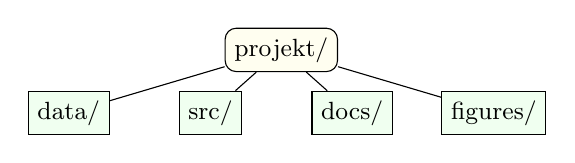
\begin{tikzpicture}[level distance=8mm, sibling distance=18mm, every node/.style={font=\small}]
            \node[draw, rectangle, rounded corners, fill=yellow!6] (root) {projekt/}
            child { node[draw, rectangle, fill=green!6] {data/} }
            child { node[draw, rectangle, fill=green!6] {src/} }
            child { node[draw, rectangle, fill=green!6] {docs/} }
            child { node[draw, rectangle, fill=green!6] {figures/} };
        \end{tikzpicture}
    \end{figure}
    \vspace{0.6em}
    Spezielle Dateien in (fast) jedem Repo:
    \begin{itemize}
        \item \texttt{README.md} (Projektbeschreibung, Anleitungen)
        \item \texttt{LICENSE} (Rechte und Nutzung)
        \item \texttt{.gitignore} (Dateien, die nicht versioniert werden sollen)
    \end{itemize}
    \begin{center}
        Beispiel: \url{https://github.com/CyrilBlum/FreeFlower}
    \end{center}
\end{frame}

% Konflikte visualisiert
\begin{frame}{Konflikte (einfach visualisiert)}
    \centering
    \begin{tikzpicture}[every node/.style={font=\small}]
        \node[draw, rectangle, fill=blue!6] (main) {main: A — B — C};
        \node[draw, rectangle, fill=green!6, below left=of main] (feat) {feature: B' — C'};
        \node[draw, rectangle, fill=red!6, below right=of main] (other) {other: B'' — C''};
        \draw[->, thick] (feat) --node[midway,below]{Merge?} (main);
        \draw[->, thick] (other) -- node[midway,below]{Merge?} (main);
        \node[below=18mm of main, font=\scriptsize] {Konflikte entstehen bei gleichzeitigen Änderungen derselben Stelle.};
    \end{tikzpicture}
\end{frame}

% Tools und Plattformen
\begin{frame}{Plattformen und Tools}
    \centering
    \begin{tikzpicture}[node distance=16mm, every node/.style={font=\small, draw, rounded corners, inner sep=3pt}]
        \node (gh) {GitHub};
        \node[below=of gh, fill=gray!6] (git) {git};
        \node[left=of git, fill=gray!6] (gui) {VSCode / GUI};
        \draw[<->] (gh) -- (git);
        \draw[<->] (gui) -- (git);
    \end{tikzpicture}
    \vspace{0.6em}
    \begin{itemize}
        \item GitHub: Remote-Hosting, Kollaboration, Issues, PRs, Wiki
        \item git: Versionskontrolle, Branching, lokale Historie
        \item VSCode / GUI: Einfache Bedienung, visuelle Darstellung von History und Diff, Integration von Git-Funktionen
    \end{itemize}
\end{frame}

% Tipps für die Maturaarbeit
\begin{frame}{Tipps für die Maturaarbeit}
    \centering
    \begin{block}{Kurz und praktisch}
        Zu jedem Meilenstein ein kurzes, aussagekräftiges Commit. Branches für Experimente. Aufbau und Data-Handling in `docs/` dokumentieren. Grosse Daten ausserhalb des Repos sichern und verlinken.
    \end{block}
\end{frame}

% Mini-Übung
\begin{frame}[fragile]{Übungen: GitHub}
    \begin{myExBox}[title={GitHub einrichten, Repo erstellen}]
        \small
        \url{https://cyrilblum.github.io/FreeFlower/github-setup.html}\\
        \qrcode{https://cyrilblum.github.io/FreeFlower/github-setup.html}
    \end{myExBox}
\end{frame}



\begin{frame}{Weiterführende Ressourcen}
    \centering
    \begin{block}{Kurz}
        Pro Git (kostenlos) und die offizielle Git-Dokumentation. GitHub Education / Students Pack. VSCode und GitHub Desktop als praktische Werkzeuge.
    \end{block}
    \vspace{0.6em}
    \begin{center}
        \Large Viel Erfolg bei der Maturaarbeit!\\
        \small Bei Interesse: Git-Workshop anbieten.
    \end{center}
\end{frame}
